%!TEX TS-program = xelatex
% !TeX program = xelatex
\documentclass{article}
\usepackage[margin=1in]{geometry}
\usepackage{xeCJK}
\usepackage{ruby}
\usepackage{pdfpages}
\usepackage{afterpage}
\setCJKmainfont{NotoSansJP-Light.otf}
\usepackage{tikz}
\usepackage{comment}
\usepackage{indentfirst}
\usepackage[linktoc=all]{hyperref}
% characters with big height and depth
% to give different boxes the same vertical size
\newcommand{\vsizecorrectorhira}{\vphantom{もりぼゃ}}% epkyouka, HanaMinA
\newcommand{\vsizecorrectorkanji}{\vphantom{$\vert$}}

% commands for setting furigana below kanji
\newcommand{\furiganaBelow}[2]{% #1: kanji, #2: furigana
    %\unskip
    \begin{tikzpicture}[baseline=(kanji.base)]
        \node(kanji)[
            inner sep=0,
        ] {
            \vsizecorrectorkanji%
            #1%
        };
        \node(furigana)[
            below of=kanji,
            node distance=1em-2pt,
            inner sep=0,
        ] {%
            \tiny%
            \vsizecorrectorhira%
            #2%
        };
    \end{tikzpicture}%
    %\ignorespaces
}

\newcommand{\furiganaAboveBelow}[3]{% #1: kanji, #2: furigana above, #3: furigana below
    %\unskip
    \begin{tikzpicture}[baseline=(kanji.base)]
        \node(kanji)[
            inner sep=0,
        ] {
            \vsizecorrectorkanji%
            #1%
        };
        \node(furigana-above)[
            above of=kanji,
            node distance=1em,
            inner sep=0,
        ] {%
            \tiny%
            \vsizecorrectorhira%
            #2%
        };
        \node(furigana-below)[
            below of=kanji,
            node distance=1em-2pt,
            inner sep=0,
        ] {%
            \tiny%
            \vsizecorrectorhira%
            #3%
        };
    \end{tikzpicture}%
    %\ignorespaces
}

\newcommand{\furigana}[2]{% #1: kanji, #2: furigana
    %\unskip
    \begin{tikzpicture}[baseline=(kanji.base)]
        \node(kanji)[
            inner sep=0,
        ] {
            \vsizecorrectorkanji%
            #1%
        };
        \node(furigana)[
            above of=kanji,
            node distance=1em-0pt,
            inner sep=0,
        ] {%
            \scriptsize%
            \vsizecorrectorhira%
            #2%
        };
    \end{tikzpicture}%
    %\ignorespaces
}

\newcommand{\tlnotelink}[1]{\hyperlink{#1tonote}{[#1]}\hypertarget{#1}{}}
\newcommand{\tlnoteref}[1]{\hypertarget{#1tonote}{}\hyperlink{#1}{[#1]}}

\setlength{\parskip}{0.4em}

\title{「心綺楼」 --- Heart, Elegance, Stage}
\author{Original Source: 凋叶棕 --- Translated by: Othi}
\begin{document}

\maketitle

\tableofcontents
\section{Origin}
\noindent Original game: 東方心綺楼 ~ Hopeless Masquerade \\
Original title: 亡失のエモーション --- Lost Emotion \\
Theme: Hata no Kokoro's (秦 こころ) theme

\section{Summary}
Sung by Kokoro and almost the whole cast of Hopeless Masquerade, main narration is by Kokoro

kokoro's dance blah blah

sect war blah blah

\begin{center}
\makebox[\textwidth]{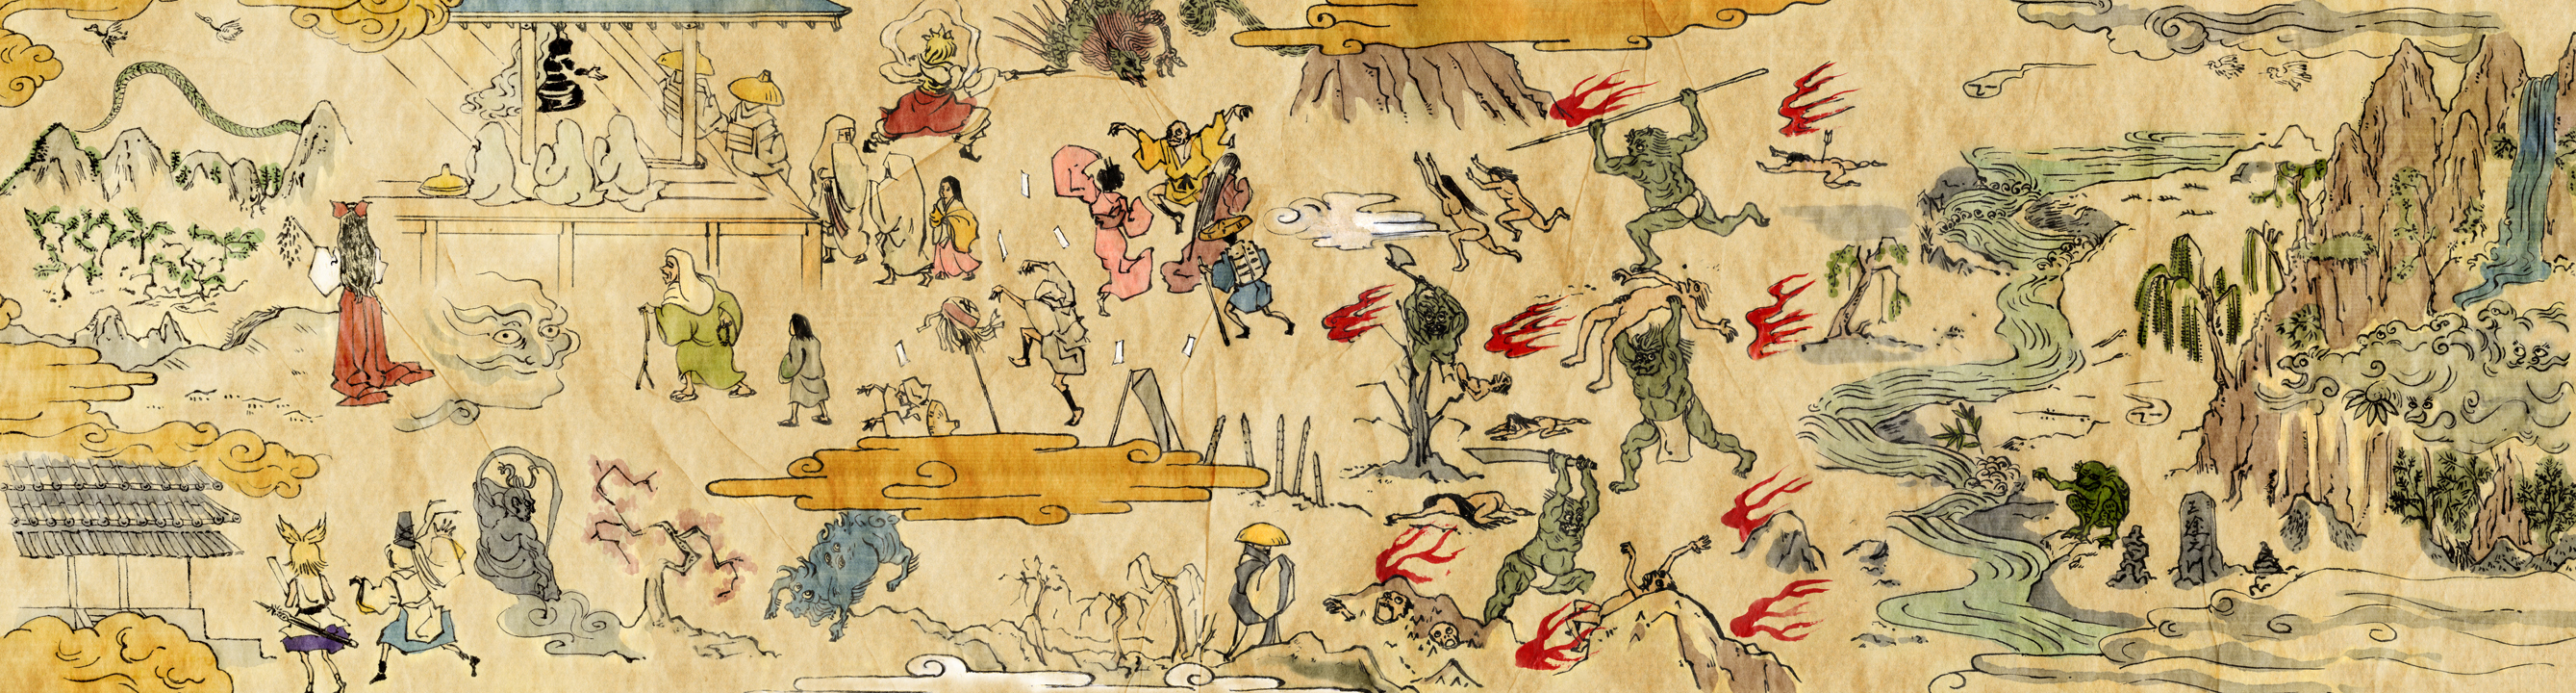
\includegraphics[width=\paperwidth,keepaspectratio]{HM_Intro_sequence.jpg}}
Hopeless Masquerade's Intro sequence, separate image in full resolution is also provided in the folder
\end{center}

\section{Lyric}
\subsection{Intro}
\furigana{生}{い}きとし\furigana{生}{い}けるものたちよ \\
To all living things, great and small

その\furigana{長}{なが}き\furigana{命}{いのち}を\furigana{以}{も}って\furigana{如何}{いか}にあるのか \\
How do you spend those long lives of yours

\furigana{悩}{なや}めど\furigana{悩}{なや}めど\furigana{答}{こた}えは\furigana{得}{え}られず \\
Even though you worry and worry without having an answer

ならば\furigana{咲}{さ}かせよ\furigana{刹那}{せつな}に\furigana{飾}{かざ}る\furigana{花}{はな} \\
If so, then mark the moment the flowers blooms

\furigana{数多}{あまた}の\furigana{感情}{おもう}よ \furigana{花}{はな}となれ---。 \\
Numerous thoughts and emotions --- Become the flower

\subsection{Verse \#1: Hakurei Reimu}
そこな\furigana{妖怪}{ようかい} \\
You youkai over there

\furigana{博麗}{はくれい}の\furigana{巫女}{みこ}の\furigana{御前}{おまえ}なら \\
You are in the presence of the Hakurei Shrine Maiden

\furigana{御}{お}\furigana{人気}{にんき}\furigana{頂戴}{ちょうだい} \\
Give me your popularity \tlnotelink{popularity}

ついでにお\furigana{賽銭}{さいせん}も\furigana{頂戴}{ちょうだい} \\
While you're at it, I can make use of some donations too

\subsection{Verse \#2: Kirisame Marisa}
\furigana{放}{はな}つ\furigana{火力}{かりょく}は \\
Such firepower

\furigana{弛}{たゆ}まぬ\furigana{日々}{ひび}の\furigana{結晶}{けっしょう}だから \\
Is the fruition of my everyday diligence

\furigana{神秘}{しんぴ}を\furigana{越}{こ}えては \\
What's no secret is

なってしまおう\furigana{希望}{きぼう}へと \\
To aim towards your goals and aspirations.

\subsection{Verse \#3: Ichirin Kumoi}
\furigana{親父}{おやじ}の\furigana{曰}{いわ}く \\
According to father

この\furigana{戦}{たたか}いの\furigana{義}{ぎ}にあってなお \\
Let this fight be fair and just

\furigana{貴様}{きさま}は\furigana{既}{すで}に \\
You have already lost

スケールの\furigana{差}{さ}で\furigana{負}{ま}けていよう \\
From the difference in scale alone

\subsection{Verse \#4: Hijiri Byakuren}
\furigana{救}{すく}おう\furigana{現世}{げんせ} \\
I'll bring salvation to this world

\furigana{最強}{さいきょう}\furigana{僧侶}{そうりょ}の\furigana{名}{な}にかけて \\
I wager on my name as the strongest monk

\furigana{力}{ちから}を\furigana{揮}{ふる}うは \\
To wield such power is to be expected

\furigana{物理的}{ぶつりてき}に\furigana{南無三宝}{なむさんぼう} \\
From the earthly treasure of the Three Jewels \tlnotelink{hijiri}

\subsection{Kokoro's 1st Part: Intro}
かき\furigana{乱}{みだ}される\furigana{信仰}{しんこう}の\furigana{在}{あ}り\furigana{方}{かた}に \\
Corrupted faith's supposed way

その\furigana{影}{かげ} \furigana{密}{みつ}か \furigana{手}{て}を\furigana{伸}{の}ばす\furigana{前}{まえ}に \\
That thick shadow reaching out its hand \tlnotelink{hopeless}

こころにまかせ \furigana{伝}{つた}えよ! \\
Leave it to the Kokoro --- I'll tell the story!

\subsection{Kokoro's 1st Part: Chorus}
この\furigana{刹那}{せつな}うつろい\furigana{行}{ゆ}く \\
This ever-changing moment

\furigana{幾重}{いくえ}\furigana{幾多}{いくた}その\furiganaAboveBelow{感情}{おもい}{かんじょう} \\
The piled up emotions

それら\furigana{平}{たい}らかならずなら \\
that certainly seems to be calm

やって\furigana{魅}{み}せよう 一\furigana{勝負}{しょうぶ}! \\
I'll make it fascinating --- Showdown!

さあ\furigana{人気}{にんき}\furigana{爆発}{ばくはつ}! \\
Now come on, eruption of popularity!

\furigana{大技}{おおわき}\furigana{激突}{げきとつ}! \\
Clashes of powerful moves

\furigana{遍}{あまね}く\furiganaAboveBelow{歓声}{こえ}{かんせい}よ---\furigana{舞台}{ぶたい}の\furigana{花}{はな}となれ。 \\
Cries of joy from afar --- Become the flower of the stage

\subsection{Verse \#5: Mononobe no Futo}
\furigana{我}{われ}は\furigana{駒}{こま}なり \\
Your servant is but a pawn

この\furigana{心}{こころ}に\furigana{曇}{くも}りなどはなく \\
There is no such thing as this heart becoming clouded or the likes

そこな\furigana{御仁}{ごじん}は---
Yours truly over there

\furigana{敵}{てき}か?! それならば\furigana{火}{ひ}を\furigana{放}{はな}て \\
Enemy huh?! Then I'll set you on fire
\subsection{Verse \#6: Toyosatomimi no Miko}
\furigana{我}{われ}から\furigana{出}{い}でよ \\
The place we come from

\furigana{遍}{あまね}く\furigana{希望}{きぼう}のある\furigana{所}{ところ}は \\
Is one of faith spreading wide and far

\furigana{新}{あらた}たな\furigana{面}{おもて} \\
This new mask \tlnotelink{mask}

これぞ\furigana{希望}{きぼう}の\furigana{形}{かたち}なり \\
Will be the figure of faith

\subsection{Verse \#7: Nitori Kawashiro}
\furigana{祭}{まつり}りとあらば \\
When there is a festival

\furigana{緩}{ゆる}む\furigana{財布}{さいふ}の\furigana{紐}{ひも}を\furigana{狙}{ねら}え \\
Gotta aim at loosened purse strings

\furigana{遊}{あそ}びじゃねえんだ \\
This is no time to play

\furigana{地獄}{じごく}の\furigana{沙汰}{さた}さえもなんとやら \\
even trials in hell have to runs on something \tlnotelink{hell}

\subsection{Verse \#8: Mamizou Futatsuiwa}
\furigana{月}{つき}が\furigana{出}{で}た\furigana{出}{で}た \\
The moon has come out

\furigana{佐渡}{さど}の\furigana{二ッ岩}{ふたついわ}のお\furigana{通}{とお}りじゃ \\
When I'm walking down the street of Sado

\furigana{人里歩}{ひとざとある}けど \\
I'm just a wandering villager

その\furigana{正体}{しょうたい}は\furigana{知}{し}れぬまま \\
But the real me won't ever be revealed

\subsection{Kokoro's 2nd Part: Verse \#1}
\furigana{次}{つぎ}から\furigana{次}{つぎ}へ\furigana{移}{うつ}ろう\furigana{信仰}{しんこう}に \\
One after another; constantly changing beliefs

\furigana{乱}{みだ}され \furigana{奪}{うば}われるその\furigana{前}{まえ}に \\
Being thrown into disorder --- stolen right in front of our eyes

こころのままに \furigana{伝}{つた}えよ! \\
As for Kokoro; I'll tell you


\subsection{Kokoro's 2nd Part: Chorus \#1}
\furigana{先}{さき}の\furigana{見}{み}えぬ\furigana{暗}{くら}がりに \\
In the darkness that can't be seen ahead

\furigana{明日}{あす}なき\furigana{命}{いのち}\furigana{送}{おく}るなら \\
To live one's life without a future

ただ\furigana{笑}{わら}って\furigana{眺}{なが}めよう \\
Just laugh and admire the view

\furigana{生}{い}きていれば ええじゃないか! \\
To be able live, isn't it already great?

さあ\furigana{人気}{にんき}\furigana{爆発}{ばくはつ}! \\
Now come on, eruption of popularity!

\furigana{弾幕}{だんまく}\furigana{炸裂}{さくれつ}! \\
Barrage of Danmaku

\furigana{飛}{と}び\furigana{交}{か}う\furiganaAboveBelow{怒号}{こえ}{どごう}よ---\furigana{舞台}{ぶたい}の\furigana{花}{はな}となれ。 \\
angry soar flying at each other --- be the flower of this stage

\subsection{Kokoro's 2nd Part: Breakdown}
\furigana{命}{いのち}は\furigana{心}{こころ}の\furigana{在}{あ}る\furigana{処}{ところ} \\
There's a heart inside everyone

\furigana{幾多}{いくた}\furigana{営}{いとな}み \\
Various performances

\furigana{人}{ひと}から\furigana{人}{ひと}へ \furigana{物}{もの}から\furigana{物}{もの}へ \\
one person after another,one creature after another

\furigana{斯}{か}く\furigana{斯}{か}くの\furigana{物語}{ものがたり} \\
Every being with stories of their own

\furigana{明日}{あした}は\furigana{行方}{ゆくえ}\furigana{知}{し}らず \\
Without knowing how future would turn out

\furigana{蜃気楼}{しんきろう}の\furigana{中}{なか} \\
Within this pessimism \tlnotelink{shinkirou}

それでも\furigana{尚}{なお}も \furigana{心}{こころ}のまま \\
Even still, this unchanging heart

\furigana{明日}{あす}へと\furigana{伝}{つた}え\furigana{行}{い}け \\
Will carry these tales towards tomorrow

\subsection{Kokoro's 2nd part: Verse \#2}
その\furigana{始}{はじ}まりより\furigana{至}{いた}るまで \\
From the beginning until the end

\furigana{全}{すべ}ての\furigana{感情}{おもい}を\furigana{見}{み}\furigana{渡}{わた}せど \\
Take a glance into every emotion

\furigana{悩}{なや}み \furigana{乱}{みだ}れて \furigana{心地}{ここち} \furigana{虚}{うつ}ろ \\
Agony; Confusion; Sensation; Emptiness

\furigana{未}{いま}だ\furigana{満}{み}ちねば \\
Those yet to have matured

\furigana{希望}{きぼう}をこの\furigana{手}{て}に!
Hope is in our grasp!

\subsection{Kokoro's 2nd part: Chorus \#2}
\furigana{宴}{うたげ}も\furigana{酣}{たけなわ}か \\
Party in full swing

\furigana{悪}{あ}しき\furigana{能}{のう}も\furigana{見納}{おさ}めよう \\
My final play coming to an end \tlnotelink{noh}

\furigana{三位一体}{さんみいったい} \furigana{調}{と}き\furigana{伏}{ふ}せて \\
I'll keep the three factions at bay

\furigana{恨}{うら}む\furigana{勿}{なか}れよ \furigana{面霊気}{めんれいき}! \\
Don't come to resent me, shroud of mystery

しかしてこちらも\furigana{負}{ま}けられぬ \\
Now I cannot afford to be defeated

\furigana{全}{すべ}ての\furigana{希望}{きぼう}がために \\
For the sake of every belief

\furigana{舞}{ま}ってみせよう\furigana{今一度}{いまいちど} \\
I'll dance for you once more

さあ'\furigana{この}{ここ}\furiganaAboveBelow{名}{ろ}{な}'の\furigana{命}{めい}ずるまま! \\
I hereby call out my name!

\furigana{人気}{にんき}\furigana{爆発}{ばくはつ}! \\
Now come on, eruption of popularity!

\furiganaAboveBelow{符乱}{スペル}{みだ}れ\furigana{飛}{と}ぶ! \\
Spells flying wildly about

\furigana{希望}{きぼう}の\furiganaAboveBelow{希求}{こえ}{ききゅう}よ---\furigana{舞台}{ぶたい}の\furigana{花}{はな}となれ。 \\
Great desire of hope --- Become the flower on this stage

---\furigana{花}{はな}となれ。 \\
--- Become the flower.

\section{Translation notes}
Sects in the religion war: Shintoism, Taoism, and Buddhism

`In the wake of so many incidents beyond their control, the Human Village has fallen into a state of hopeless pessimism. Believing that religion can restore order, some of Gensokyo's most prominent adherents of Buddhism, Taoism and Shinto all want to take this chance to expand their particular faith's influence.' -\href{https://en.touhouwiki.net/wiki/Hopeless_Masquerade#Plot}{Touhou Wiki}


Todo:

- simile and parallel between hope and faith (gensokyo faith)

- chorus and koe transformation from the lyrics

- context for popularity

\tlnoteref{hopeless}: hopelessness and pessimism from the human village in the wake of numerous incidents beyond their control, the black fog can be both the youkai's shadow or the humans' negative energy

\tlnoteref{popularity}: using popularity in this context throughout the whole song sounds extremely weird at least to my opinion, I've tried to think of other alternatives but to no avail, because not only there is already so few synonyms to popularity, but also how popularity is in fact a core mechanic in the game and there really is no other equivalent. The goal of the religion war was in fact a fight for popularity after all, with all three fighting to be the most popular and beloved religion when the incidents at the Human Village were taking place, hence I've decided to leave it as is.

\tlnoteref{shinkirou}: 蜃気楼 and 心綺楼 are pronounced the same (しんきろう). The meaning of the word is mirage, but I decided to translate it as shroud of desperation as in Japanese this is a wordplay to both mean mirage (蜃気楼) --- an object shrouded in uncertainty/mist/illusion and hopeless masquerade (心綺楼) --- the game's title

\tlnoteref{hijiri}: referencing herself, saying she is the physical manifestation of the Homage to the Three Jewels. Real life Three Jewels consists of Buddha, Dharma and Sangha \href{https://en.wikipedia.org/wiki/Refuge_(Buddhism)}{Source}

\tlnoteref{noh}: Note on the word 能 --- Kokoro's performance in the human village

舞台: Noh stages

\tlnoteref{hell}: This is the intentionally botched idiom 地獄の沙汰も金次第 (じごくのさたもかねしだい): money talks; money is the best lawyer in hell; even the verdict of hell is determined by money

\tlnoteref{mask}: this is the symbol to the most ancient noh mask given from the legendary prince Shoutoku who is Miko's based off of. \href{en.wikipedia.org/wiki/Noh#Masks}{Source}

Own note: has everyone's POV in hopeless masquerade except for Koishi

Everyone's including Kokoro's (albeit Kokoro's is a bit more monotone and straightfoward due to both of her personality as a extremely monotone character and also having the role of the narrator in this play) pattern of speech are different, translation with also an aim to deliver the correct context and characterization is essential
\end{document}
